\chapter{Grundlagen}
\label{chap:grundlagen}
% TODO ggf. TP, FN, FP, TN erklären und auch f1 score, f Score
In \autoref{sec:software-zitation} wird auf die Prinzipien der Software-Zitation eingegangen.
Es wird beschrieben, warum die Zitation von Software ebenfalls wichtig ist, ähnlich wie die Zitation von anderen wissenschaftlichen Arbeiten.
Außerdem wird darauf eingegangen, dass ebenfalls Personen zitiert werden sollten, welche nicht aktiv an der Software programmieren.
Zusätzlich dazu wird in \autoref{sec:autorenrolle-oss} auf die Rolle von Autoren in \gls{oss} eingegangen und ein wissenschaftliches Paper dargestellt, welches dies bereits analysiert hat.

Autoren von Software werden in unterschiedlichen Quellen zitiert.
Einige dieser Quellen sind stark mit der Softwareentwicklung verbunden.
Es existieren verschiedene Systeme, die Entwicklern zur Verfügung stehen, um ihre Arbeit effizienter zu gestalten oder überhaupt praktikabel zu machen.
In diesen Systemen können Sie außerdem als Autoren genannt werden.
In den Abschnitten \ref{sec:versionsverwaltung} und \ref{sec:paketverwaltung} wird auf die Versions- und Paketverwaltung eingegangen, welche zwei dieser Systeme darstellen.
Des Weiteren existieren spezielle Zitierformate, in welchen Autoren explizit angegeben werden können.
Auf diese Formate wird in \autoref{sec:zitierformate} eingegangen.
Zudem können in Fließtexten, beispielsweise der Beschreibung einer Software, ebenfalls Autoren genannt werden.
In \autoref{sec:named-entity-recognition} wird auf die \emph{Named Entity Recognition} eingegangen, welche eine Methode darstellt, um Personen in Texten zu erkennen.

Alle Quellen, welche beschrieben werden, dienen im Verlauf der Masterarbeit als Grundlage für die Extraktion von Autoren und deren Metainformationen.
Die extrahierten Autoren müssen anschließend zugeordnet werden.
Der Prozess dafür heißt \emph{Author Name Disambiguation}, welcher in \autoref{sec:author-name-disambiguation} beschrieben wird.
Eine weitere Möglichkeit des Abgleichs ist ein Abgleich von Zeichenfolgen.
Dieser funktioniert jedoch nicht immer, da Autoren unterschiedliche Schreibweisen ihres Namens verwenden können.
Aus diesem Grund wird in \autoref{sec:unscharfe-suche} auf die unscharfe Suche eingegangen, welche eine Möglichkeit darstellt, um ähnliche Zeichenfolgen miteinander zu vergleichen, beispielsweise für den Abgleich von Namen mit oder ohne genannten Zwischennamen.
\section{Zitation von Software}
\label{sec:software-zitation}
Software ist ein wesentlicher Bestandteil moderner Forschung.
In der wissenschaftlichen Literatur ist es üblich, Quellen zu zitieren, um die Nachvollziehbarkeit und Reproduzierbarkeit von wissenschaftlichen Arbeiten zu gewährleisten.
Im Gegensatz dazu ist dies bei wissenschaftlicher Software aktuell in diesem Umfang noch nicht gegeben.
Hier gibt es aktuell kaum Anerkennung und Unterstützung für die Leistungen einzelner Autoren.
Aus diesem Grund hat die \glqq FORCE11 Software Zitier Arbeitsgruppe\grqq{} Prinzipien der Software Zitation erstellt, welche eine breite Akzeptanz in der wissenschaftlichen Gemeinschaft finden sollen.
Im Folgenden werden die Prinzipien vorgestellt und erläutert \cite{smith_software_2016}:

\begin{enumerate}
    \item \textbf{Wichtigkeit:} Software sollte ein seriöses und zitierbares Produkt wissenschaftlicher Arbeit sein. Software Zitierungen sollten im wissenschaftlichen Kontext die gleiche Bedeutung zugeschrieben bekommen wie Zitierungen anderer Forschungsprodukte, wie Publikationen. Sie sollten wie Publikationen auch in der Arbeit enthalten sein, zum Beispiel in der Referenzliste eines Artikels. Software sollte auf derselben Grundlage zitiert werden wie jedes andere Forschungsprodukt auch, wie zum Beispiel ein Aufsatz oder ein Buch. Das bedeutet, dass Autoren die entsprechend verwendete Software zitieren sollten, so wie sie die entsprechenden Publikationen zitieren würden.
    \item \textbf{Anerkennung und Zuschreibung:} Softwarezitate sollten die wissenschaftliche Anerkennung und die normative, rechtliche Würdigung aller Mitwirkenden an der Software ermöglichen, wobei anerkannt wird, dass ein einziger Stil oder ein Mechanismus für die Namensnennung nicht auf jede Software anwendbar sein kann.
    \item \textbf{Eindeutige Identifikation:} Ein Softwarezitat sollte eine Methode zur Identifikation enthalten, die maschinell verwertbar, weltweit eindeutig und interoperabel ist und zumindest von einer Gemeinschaft der entsprechenden Fachleute und vorzugsweise von allgemeinen Forschern anerkannt wird.
    \item \textbf{Persistenz:} Eindeutige Identifikatoren und Metadaten, die die Software und ihre Verwendung beschreiben, sollten bestehen bleiben – auch über die Lebensdauer der Software hinaus, die sie beschreiben.
    \item \textbf{Zugänglichkeit:} Softwarezitate sollten den Zugang zur Software selbst und zu den zugehörigen Metadaten, Dokumentationen, Daten und anderen Materialien erleichtern, die sowohl für Menschen als auch für Maschinen notwendig sind, um die referenzierte Software sachkundig nutzen zu können.
    \item \textbf{Spezifizität:} Softwarezitate sollten die Identifizierung und den Zugang zu der spezifischen Version der verwendeten Software erleichtern. Die Identifizierung der Software sollte so spezifisch wie nötig sein, z. B. durch Versionsnummern, Revisionsnummern oder Varianten wie Plattformen.
\end{enumerate}

In dieser Arbeit wird verstärkt auf das Prinzip der Wichtigkeit eingegangen, da besonders im \gls{cff} und Bib\TeX{} Format die Möglichkeit besteht nicht die Software, sondern beispielsweise ein Artikel anzugeben.
Diese Zitierweise würde dann das Prinzip der Wichtigkeit verletzen, da die Software nicht die gleiche Bedeutung zugeschrieben bekommt wie andere Forschungsprodukte.
Diese Diskrepanz wird in \autoref{chap:ergebnisse} dargestellt.

Es gibt verschiedene Gründe, warum die Zitation von Software ebenfalls wichtig ist und auch, dass Standards der Zitation eingehalten werden, ähnlich wie es der Fall bei anderen wissenschaftlichen Arbeiten ist.
Einige dieser Gründe werden im Folgenden genannt \autocite{smith_software_2016}:

\begin{itemize}
    \item Forschungsfelder verstehen: Software ist ein Produkt der Forschung und wenn sie nicht zitiert wird, werden Lücken in der Aufzeichnung der Forschung über den Fortschritt in diesem Forschungsfeld entstehen.
    \item Anerkennung: Akademische Forscher auf allen Ebenen, einschließlich Studenten, Postdocs, Dozenten und Mitarbeiter, sollten für die Softwareprodukte, die sie entwickeln und zu denen sie beitragen, anerkannt werden, insbesondere wenn diese Produkte die Forschung anderer ermöglichen oder fördern. Nicht-akademische Forscher sollten ebenfalls für ihre Softwarearbeit anerkannt werden, obwohl die spezifischen Formen der Anerkennung sich von denen für akademische Forscher unterscheiden.
    \item Software entdecken: Mithilfe von Zitaten kann die in einem Forschungsprodukt verwendete Software gefunden werden. Weitere Forscher können dann dieselbe Software für andere Zwecke verwenden, was zu einer Anerkennung der für die Software Verantwortlichen führt.
    \item Reproduzierbarkeit: Die Angabe der verwendeten Software ist für die Reproduzierbarkeit notwendig, aber nicht ausreichend. Zusätzliche Informationen wie Konfigurationen und Probleme auf der Plattform sind ebenfalls erforderlich.
\end{itemize}

Wie bereits erwähnt werden Autoren in unterschiedlichen Quellen angegeben.
Einige dieser Quellen werden in dieser Masterarbeit untersucht, wie beispielsweise das \gls{cff} und Bib\TeX{} Format.
Die Autoren in diesen Quellen werden von dem jeweiligen Softwareprojekt angegeben.
Falls an dem Projekt nicht nur Softwareentwickler beteiligt sind, sondern beispielsweise auch Grafikdesigner oder Übersetzer, so sollten diese ebenfalls in den Quellen angegeben werden.
Dies ist wichtig, da diese Personen ebenfalls einen Beitrag zum Projekt geleistet haben und somit auch Anerkennung verdienen.

Es gibt ebenfalls bereits Projekte, welche sich für die halb automatische Nennung von Autoren ohne Code Beitrag einsetzen.
Ein Beispiel für ein solches Projekt ist \glqq All Contributors\grqq{} \autocite{all_contributors_recognize_2024}.
Bei der Verwendung von \glqq All Contributors\grqq{} werden die Mitwirkenden jedoch nicht in einem speziellen Format angegeben, sondern standardmäßig in der README-Datei, welche im Projekt enthalten ist.
Die Liste wird dabei von einem Bot automatisch generiert und aktualisiert, sodass sie der Spezifikation von \glqq All Contributors\grqq{} entspricht.
Über einen Befehl in einem Issue oder einem Pull Request kann ein neuer Mitwirkender hinzugefügt werden.
Autoren, welche keinen Code beigetragen haben, stellen im weiteren Verlauf der Masterarbeit ein Problem dar, da diese nicht mit den Autoren aus den Quellen abgeglichen werden können, da sie keine Commits haben.
Dies wird in \autoref{sec:abgleich} genauer erläutert.

% TODO darauf noch eingehen? https://google.github.io/opencasebook/authorship/
Die untersuchten Pakete in dieser Arbeit sind Open Source, welche auf GitHub veröffentlicht werden.
Open Source Software ist Software, deren Quellcode öffentlich zugänglich ist und von einer Gemeinschaft von Entwicklern entwickelt wird.
Die Entwickler arbeiten dabei in der Regel ehrenamtlich und ohne Bezahlung an der Software, wobei einige der untersuchten Pakete auch von Organisationen veröffentlicht werden, wie beispielsweise die \glqq google-auth-library-python
\grqq{} von Google.
Diese wird primär von Google Mitarbeitern entwickelt und gepflegt.
Wie bereits beschrieben sind Prinzipien und Gründe definiert, warum Software ebenfalls zitiert werden sollte.
Welche Autoren in den Quellen angegeben werden sollten, ist jedoch nicht so genau definiert wie es beispielsweise im Bereich von wissenschaftlichen medizinischen Artikel der Fall ist.
In diesem Bereich hat das \glqq International Commitee of Medical Journal Editors\grqq{} Richtlinien für die Rolle von Autoren und Beitragenden in wissenschaftlichen Artikeln definiert \autocite{noauthor_icmje_nodate}.
Unter anderem aus diesem Grund ist die Menge der Autoren, welche in den Quellen angegeben werden, unterschiedlich und hängt von dem jeweiligen Projekt ab.
Außerdem ist es möglich, dass ausschließlich Autoren in den Quellen angegeben werden, welche aktuell nicht mehr an dem Projekt beteiligt sind, aber beispielsweise vor fünf Jahren aktiv das Projekt geführt haben.
Diese und weitere Auffälligkeiten werden in der Masterarbeit untersucht.
Auch dies ist in anderen Bereichen anders definiert, sodass auch die neuen Autoren genannt werden müssen wie beispielsweise bei Neuauflagen von Büchern.

\section{Autorenrolle und Anerkennung in Open-Source-Software}
\label{sec:autorenrolle-oss}
% TODO ggf. noch mehr schreiben?
% TODO ggf. weitere Paper?
In der Wissenschaft existieren bereits Analysen zur Rolle von Autoren in \gls{oss}.
Ein Paper analysiert die Zuschreibung von Entwicklern in \gls{oss} \autocite{young_which_2021}.
Sie beantworten in dem Paper folgende Fragen:

\begin{itemize}
  \item Wie unterscheiden sich die Modelle für die Anerkennung von Beiträgen?
  \item Wie viele Informationen gehen verloren, bei einer Festlegung auf Repository-Änderungen als Modell für den Beitrag?
  \item Wie entwickeln sich die Beiträge zu \gls{oss} über die Zeit?
  \item Können wir Projekte auf der Grundlage von Beitragsmustern klassifizieren?
\end{itemize}

In dem Paper werden vier Modelle für die Anerkennung unterschieden.
Im ersten Modell werden die Änderungen an einem Repository als Beitrag betrachtet.
Dabei wird auf die Top 100 Benutzer in den Projekten geschaut, wie sie durch die GitHub API ausgegeben werden.
Das zweite Modell betrachtet die Autoren, welche automatisch über ein Tool identifiziert werden.
In dem Paper wird hierbei das Programm \textit{octohatrack} verwendet \autocites{young_which_2021}{noauthor_labhroctohatrack_2024}.
Als drittes Modell werden die Autoren mittels Taxonomien identifiziert.
Hierbei wird die \mintinline{text}{.all-contributorsrc}-Datei von \glqq All Contributors\grqq{} analysiert \autocites{young_which_2021}{all_contributors_recognize_2024}.
Das vierte Modell betrachtet die Autoren, welche mittels ad hoc Methoden identifiziert werden.
Diese können beispielsweise durch die Analyse von nicht standardisierten Quellen stammen wie beispielsweise Webseiten oder unstrukturierten Textdateien.
Das Modell wird in dem Paper aufgrund der Komplexität nicht fokussiert betrachtet.

Die Autoren betrachten die Fragen und Modelle dabei von einer gehobenen Perspektive.
Dabei werden die einzelnen Fragen mithilfe von verschiedenen generellen Metriken wie die Anzahl der Autoren, welche Commits erstellt haben oder als Autoren in \glqq All Contributors\grqq{} genannt werden, beantwortet.
Sie betrachten keine einzelnen Autoren oder Projekte, sondern analysieren die gesamte \gls{oss}-Landschaft primär auf Basis von der Anzahl der Autoren.
Es werden keine genaueren Analysen durchgeführt wie beispielsweise in dieser Masterarbeit, in der unter anderem betrachtet wird, ob die genannten Autoren noch aktiv an dem Projekt beteiligt sind.
Außerdem wird nicht auf Daten eingegangen, welche aus weiteren Quellen wie dem \gls{cff} oder \hologo{BibTeX} Format stammen.

\section{Versionsverwaltung}
\label{sec:versionsverwaltung}
% TODO Das ändern ist erstmal nur kopiert und auch anpassen wie zitiert wird er mag es nicht wenn ganze abschnitte eine quelle haben. Immer nur den Teil der wirklich aus der Quelle ist zitieren
% TODO noch mehr schreiben sollte auf 3 Seiten kommen
% TODO Issue und Pull Request in der Versionsverwaltung erwähnen und erklären
% TODO auf Github eingehen was das ist und wofür das benutzt wird
Die Versionsverwaltung ist ein System, um verschiedene Versionen von Software zu verwalten.
Es bietet Zugang zu Code und dessen Änderungen in der Vergangenheit.
Der Code und getätigte Änderungen werden in einem Repository gespeichert.
Dadurch ist die Versionsverwaltung eine Art Logbuch, in dem alle Änderungen festgehalten werden.
Dabei wird zusätzlich zu der Änderung der Autor und der Zeitpunkt der Änderung festgehalten.
Dies ermöglicht es in dem Forschungsseminar empirisch die Menge an Arbeit der einzelnen Autoren zu ermitteln. \autocite{ponuthorai_version_2022}

Es gibt zwei verschiedene Arten von Versionsverwaltungssystemen.
Zum einen gibt es die zentralen Systeme, bei denen alle Änderungen zentral verwaltet werden, beispielsweise SVN.
Zum anderen gibt es die verteilten Systeme, bei denen jeder Entwickler eine Kopie des gesamten Repository und dessen Vergangenheit hat.
Ein solches System ist Git, welches sich mit einem Marktanteil von ungefähr 75 \% gegenüber anderen Systemen durchgesetzt hat \autocite{lindner_version_2024}.
Aus diesem Grund und weil Git-Repositorys in der Arbeit untersucht werden, wird auf Git eingegangen.
Dabei werden Begriffe erklärt, mit denen es möglich ist, die geleistete Arbeit von einzelnen Autoren innerhalb eines Repositorys zu untersuchen. \autocite{ponuthorai_version_2022}

In Repositorys gibt es verschiedene Arten von Statistiken.
In Git werden Revisionen als ein \emph{Snapshot} gespeichert.
Anders als in anderen Systemen wird keine Serie von Änderungen gespeichert, sondern ein \emph{Snapshot} der Änderungen zu einem bestimmten Zeitpunkt erstellt.
Dies wird ein Commit genannt.
An einem Commit werden verschiedene Metainformationen gespeichert.
Unter anderem wird eine Commit-Nachricht, der Autor und der Zeitpunkt der Änderungen gespeichert.
Mehrere Commits bilden die Commit-Historie bzw. die Vergangenheit eines Repositorys.
Weitere Eigenschaften, welche sich aus dem Repository exportieren lassen, sind die Anzahl der eingefügten und gelöschten Zeilen.
Außerdem lässt sich die Anzahl der geänderten Dateien ermitteln.
Diese Werte können für das gesamte Repository oder für einzelne Autoren ermittelt werden. \autocite{ponuthorai_version_2022}

Die Statistiken der Repositorys können auf verschiedene Arten aufgearbeitet werden.
Zum einen können einige direkt mittels Git-Befehlen ausgelesen werden \autocite{chacon_git_2024}.
Andere wiederum benötigen komplexere Abfragen, welche beispielsweise mittels Skripten oder speziellen Programmen ausgelesen werden können.
Ein Beispiel für ein Programm, welches Git-Statistiken aufarbeitet, ist \emph{git-quick-stats} \autocite{mestan_git-quick-stats_2024}.
Außerdem bieten Onlinedienste zur Versionsverwaltung, wie GitHub, Statistiken über APIs an, welche jedoch im Umfang der Anfragen limitiert sind \autocite{github_rate_2022}.

\section{Software-Verzeichnisse und Paketverwaltung}
\label{sec:paketverwaltung}
Im Gegensatz zur Versionsverwaltung verwaltet die Paketverwaltung keinen Code und dessen Änderungen, sondern fertige Softwarepakete, welche von Entwicklern erstellt und in einem Software-Verzeichnis abgelegt werden.
Inhalt eines Pakets können beispielsweise standardisierter Code von Software-Modulen sein oder kompilierter Code.
Zusätzlich werden in einem Paket Metadaten gespeichert.
Diese Metadaten können beispielsweise eine Beschreibung, Version, Abhängigkeiten und Autoren des Pakets enthalten.
Sie lassen sich aus dem Paket mithilfe des Paketverwaltungssystems auslesen oder über APIs des Software-Verzeichnisses abrufen.
Außerdem übernimmt das Paketverwaltungssystem das Installieren und meistens auch das Aktualisieren und Deinstallieren von Paketen.
Zusätzlich wird das System verwendet, um fehlende Abhängigkeiten von Paketen automatisch zu installieren \autocite{spinellis_package_2012}.

In dieser Arbeit wird auf zwei Software-Verzeichnisse eingegangen.
Zum einen wird auf \gls{pypi} eingegangen, welches das Verzeichnis für Python ist und von der Paketverwaltung \emph{pip} verwendet wird.
Zum anderen wird auf \gls{cran} eingegangen, welches das Verzeichnis für R ist.
In \gls{pypi} sind aktuell mehr als 500.000 unterschiedliche Projekte mit über 5 Millionen Veröffentlichungen verfügbar \autocite{python_software_foundation_pypi_2024}.
Im Gegensatz dazu sind in \gls{cran} aktuell mehr als 20.000 Pakete verfügbar \autocite{cran_team_comprehensive_2024}.

\subsection{PyPI}
\label{subsec:paketverwaltung_pypi}
\gls{pypi} hat zu Beginn des Jahres 2024 ein \gls{pep} veröffentlicht, welches die Verifizierung von Daten auf \gls{pypi} beschreibt \autocite{python_software_foundation_pep_2024}.
In dem \gls{pep} werden Änderungen an der API beschrieben, welche zum Hochladen von Paketen genutzt wird, um sogenannte \glqq Attestation objects\grqq{} zu unterstützen, in denen digitale Signaturen enthalten sind.
Das Ziel ist es verifizierte Daten auf \gls{pypi} zu ermöglichen, sodass Anwender direkt erkennen können, ob die Daten vertrauenswürdig sind.
Aktuell wird dieses \gls{pep} umgesetzt, wodurch es zu vielen Änderungen in der API und auch in der Weboberfläche von \gls{pypi} kommt.

Außerdem sind noch nicht alle Daten über die APIs erreichbar und es ist auch aktuell nicht über die API erkennbar, ob es sich um verifizierte oder nicht verifizierte Daten handelt.
Ein Beispiel für verifizierte Daten sind Links, beispielsweise zu GitHub.
Diese Links werden von \gls{pypi} als verifiziert angesehen, wenn der Upload des Pakets auf \gls{pypi} über eine GitHub-Action erfolgt.
Zudem werden die Personen als verifiziert dargestellt, welche in \gls{pypi} als Owner oder Betreuer des Pakets eingetragen sind, sie haben somit einen Account bei \gls{pypi}.
Der dargestellte Owner kann nicht über eine API abgefragt werden.

Die dargestellten GitHub-Statistiken werden dabei von \gls{pypi} ermittelt und nicht über APIs ausgegeben.
Das Ziel von \gls{pypi} ist es, dass alle Daten verifiziert werden können und keine Daten in der unverifizierten Form vorliegen.

\begin{figure}
    \begin{center}
        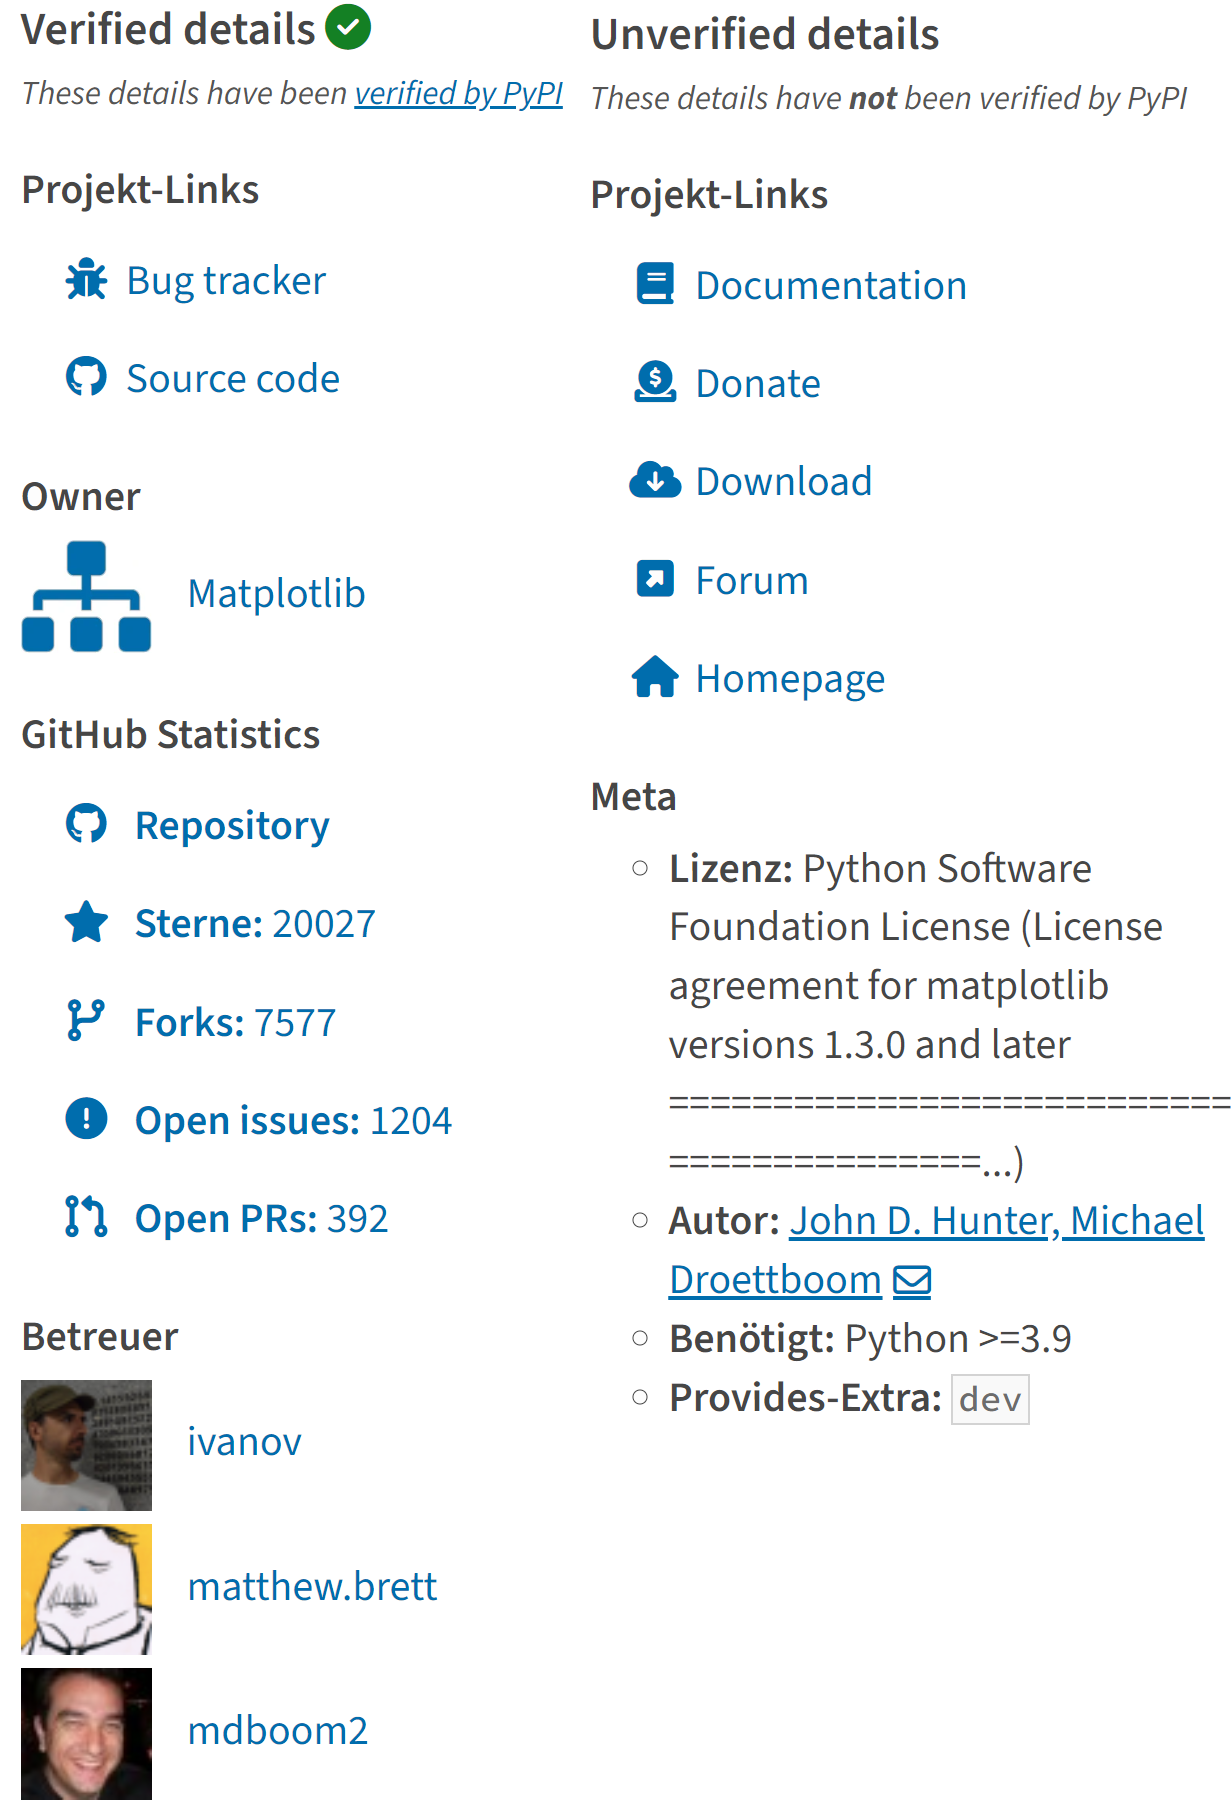
\includegraphics[width=0.95\textwidth]{bilder/pypi.png}
    \end{center}
    \caption{\gls{pypi} Verifizierte und unverifizierte Daten}
    \label{fig:pypi_verified_unverified_details}
    \small
    Die Abbildung stellt die verifizierten und unverifizierten Daten des Pakets \emph{matplotlib} auf \gls{pypi} dar \autocite{python_software_foundation_pypi_2024}.
\end{figure}

\gls{pypi} bietet verschiedene APIs und Quellen an, um die Daten der Pakete abzufragen.
Im Folgenden werden auf einige der Zugriffsmöglichkeiten eingegangen, welche mit Ausnahme der BigQuery alle in dieser Arbeit verwendet werden.

\subsubsection*{JSON-API}
\label{subsubsec:pypi_json_api}
% TODO ggf. die nicht verifizierten Daten stammen aus der Python toml (stammen die Daten wirklich alle aus der toml?) Falls ja das erwähnen und erklären, dass die Daten direkt von dem Python-Paket stammen und pypi diese nur durchreicht
Die JSON-API ist die bevorzugt zu verwendende API von \gls{pypi} und bietet die Möglichkeit, die Metadaten eines Pakets abzufragen \autocite{python_software_foundation_warehouse_2024}.
Diese API ist nicht in der Anzahl der Anfragen beschränkt.
Daten der neuesten Version des Pakets werden von der API zurückgegeben.
Die Werte in den Metadaten stammen aus den Daten, welche beim Hochladen auf \gls{pypi} angegeben wurden.
Die Daten des ersten Uploads eines Releases werden dabei als Metadaten der Version gespeichert und bei weiteren Uploads dieser Version nicht überschrieben.

Inhalt der Metadaten sind beispielsweise die Autoren und Maintainer zuzüglich deren E-Mail-Adresse, die Beschreibung, Lizenz und Links zu unterschiedlichen Quellen, beispielsweise einem GitHub-Repository \autocite{python_software_foundation_warehouse_2024}.
Die Beschreibung kann den Text aus der README-Datei des Pakets auf GitHub enthalten.
Es ist jedoch auch möglich, eine eigene Beschreibung für \gls{pypi} anzugeben, sodass sich die README-Datei in GitHub und die Beschreibung auf \gls{pypi} unterscheiden können.
Die Metadaten werden von den Entwicklern des Pakets eingetragen.
In \autoref{fig:pypi_verified_unverified_details} sind einige der Metadaten des Pakets \emph{matplotlib} unter dem Punkt \glqq Meta\grqq{} dargestellt.
Weitere Daten sind unter dem Punkt \glqq Projekt-Links\grqq{} unter den verifizierten Details dargestellt.

Die Autoren und Maintainer aus den Metadaten müssen nicht den verifizierten Betreuern und Owner des Pakets auf \gls{pypi} entsprechen, da dies unterschiedliche Systeme sind.
Zum einen sind es die Benutzer, welche Rechte auf \gls{pypi} haben, um das Paket dort anzupassen und zum anderen sind es die Personen, welche durch die Entwickler des Pakets angegeben werden.
Die Autoren und Maintainer können jedoch ebenfalls verifiziert sein, wobei dies über die API noch nicht abgefragt werden kann, jedoch in der Weboberfläche bereits für einige Pakete dargestellt wird.
Es gibt aktuell wenig Pakete, bei denen die Autoren verifiziert sind, ein Beispiel ist das Paket \emph{hololinked}, welches zum Zeitpunkt des Schreibens darüber verfügt.
\emph{Matplotlib} unterstützt dies aktuell noch nicht, wie in \autoref{fig:pypi_verified_unverified_details} dargestellt ist.
Die verifizierten Betreuer und Owner können aktuell nicht über die JSON-API abgefragt werden, sondern müssen über die XML-RPC-API abgefragt werden, da diese die einzige API ist, welche die Daten zur Verfügung stellt.

\subsubsection*{PyPI XML-RPC}
\label{subsubsec:pypi_xml_rpc}
Die \gls{pypi} XML-RPC-API ist eine veraltete API, welche jedoch noch genutzt werden kann, um einige Informationen zu den Paketen abzufragen.
Es wird empfohlen, diese API nicht mehr zu verwenden und auf den RSS-Feed oder die JSON-API umzusteigen \autocite{python_software_foundation_warehouse_2024}.
Dadurch ist die API in der Anzahl der möglichen Anfragen stark limitiert und auch die Abstände zwischen den Anfragen müssen relativ groß sein.
\gls{pypi} macht keine genauen Angaben darüber, wie viele Anfragen in welchem Zeitraum möglich sind.
Diese API ist jedoch die einzige Quelle, um die Betreuer eines Pakets abzufragen, ohne einen Web-Scraper einsetzen zu müssen.
Web-Scraping bezeichnet dabei das Extrahieren von Daten aus Webseiten, indem der HTML-Code der Webseite analysiert wird \autocite{richardson_beautifulsoup4_2024}.

Die Betreuer, welche über die API ausgegeben werden, enthalten den Benutzernamen auf \gls{pypi}, ein Vollname wird hierbei nicht ausgegeben.
Außerdem enthalten sie eine Rollenbezeichnung, welche entweder \emph{Maintainer} oder \emph{Owner} sein kann, welcher in der Oberfläche nicht dargestellt wird.
Owner können dabei alle Änderungen am \gls{pypi} Projekt vornehmen und Betreuer können neue Versionen des Pakets veröffentlichen \autocite{ingram_deprecate_2023}.
Der Benutzername für die Betreuer des Pakets \emph{matplotlib} sind in \autoref{fig:pypi_verified_unverified_details} unter dem Punkt \glqq Betreuer\grqq{} dargestellt.
Aktuell stellt \gls{pypi} keine API bereit, um den Namen eines Benutzers abzufragen, sodass nur der Benutzername über eine API abgefragt werden kann \autocite{python_software_foundation_add_2024}.

\subsubsection*{BigQuery}
\label{subsubsec:pypi_bigquery}
Ebenfalls bietet \gls{pypi} über Google BigQuery einen Datensatz an, in dem alle Pakete mit ihren Versionen und Metadaten enthalten sind \autocite{python_software_foundation_warehouse_2024}.
BigQuery ist ein Dienst von Google, welcher auf der Infrastruktur der Google Cloud-Plattform ausgeführt wird \autocite{google_bigquery_2024}.
Es ist möglich, den kompletten Datensatz auf BigQuery in mehreren einzelnen CSV-Dateien herunterzuladen.
Dabei kann ausgewählt werden, welche Daten heruntergeladen werden sollen.

Nicht alle Metadaten, welche über die JSON-API abgefragt werden können, stehen in der BigQuery zur Verfügung.
Ebenfalls stehen nicht alle Daten der BigQuery in der JSON-API zur Verfügung.
Die wichtigsten Daten sind in beiden Quellen enthalten.
So sind beispielsweise der Autor und Maintainer und deren E-Mail-Adressen in beiden Quellen enthalten.
Auch die Beschreibung, Version und Abhängigkeiten sind in beiden Quellen enthalten.
Die jeweiligen Daten, wie die Autoren eines Pakets, sind in beiden Quellen identisch.

\subsection{CRAN}
\label{subsec:paketverwaltung_cran}
\gls{cran} selbst bietet keine API an, um die Metadaten der Pakete abzufragen.
Jedoch gibt es das METACRAN-Projekt, welches eine Kollektion von kleinen Diensten für das \gls{cran}-Repository bereitstellt.
Eines dieser Dienste ist eine API, welche die \gls{cran} Downloads bereitstellt.
Über diese API ist es unter anderem möglich, eine Liste der meist heruntergeladenen Pakete in einem bestimmten Zeitraum abzufragen \autocite{csardi_cranlogsapp_2024}.
Ein weiterer Dienst, welcher durch das METACRAN-Projekt bereitgestellt wird, ist eine CouchDB, welche die Metadaten aller Pakete von \gls{cran} bereitstellt.
Dieser Dienst wird ebenfalls von dem R-Paket \emph{pkgsearch} genutzt, welches dazu dient, in R die Metadaten anderer Pakete abzufragen.
Die beiden Projekte sind keine \gls{cran} Projekte, was bedeutet, dass sie nicht von den Entwicklern von \gls{cran} betrieben werden.
Eine CouchDB ist eine Apache-Datenbank, welche nativ eine HTTP/JSON-API bereitstellt \autocite{the_apache_software_foundation_apache_2024}.
Die Datenbank ist eine Kopie des \gls{cran}-Repository und wird regelmäßig aktualisiert \autocite{csardi_pkgsearch_2023}.

Um in \gls{cran} ein Paket hinzufügen zu können, muss ein Formular ausgefüllt werden.
Dabei muss der eigene Name sowie eine E-Mail-Adresse und das Paket angegeben werden.
Anschließend werden die Daten von einem teilweise automatisierten Prozess überprüft und nach einer erfolgreichen Überprüfung wird das Paket in \gls{cran} veröffentlicht \autocite{altmann_comprehensive_2024}.
Aus diesem Grund gibt es in \gls{cran} keine Unterscheidung zwischen verifizierten und nicht verifizierten Daten, da sie im Gegensatz zu \gls{pypi} manuell geprüft werden.

Die Metadaten der einzelnen Pakete, welche über die METACRAN-API erreichbar sind, sind dabei ähnlich zu denen in \gls{pypi} \autocite{csardi_pkgsearch_2023}.
Es werden beispielsweise die Autoren, Maintainer, eine Beschreibung, die Version und Abhängigkeiten über die API ausgegeben.
Die Autoren werden in zwei unterschiedlichen Formaten ausgegeben.
Zum einen wird ein Feld \glqq Author\grqq{} ausgegeben, welches die Autoren in einer Zeichenfolge enthält.
Dieses Feld enthält den Namen der Autoren, sowie ggf. deren Rolle und ORCID iD.
Zum anderen wird ein Feld \glqq Authors@R\grqq{} ausgegeben, welches die Autoren in einem R-Format ausgibt.
Dieses Feld enthält ebenfalls die Werte des Feldes \glqq Author\grqq{}, sowie ggf. eine E-Mail-Adresse des jeweiligen Autors. 
Im Gegensatz zu \gls{pypi} gibt es bei \gls{cran} keine Benutzer für das Software-Verzeichnis.
Außerdem lassen sich alle Metadaten über die gleiche API abfragen.
Es wurden keine Informationen über mögliche Limitierungen in der Anzahl der Anfragen gefunden.

\section{Zitierformate}
\label{sec:zitierformate}
In diesem Abschnitt wird auf unterschiedliche Zitierformate eingegangen, welche die Datenstruktur hinter einer Zitation beschreiben.
In dieser Arbeit wird sich auf das \gls{cff} und das \hologo{BibTeX}-Format beschränkt.
Das \gls{cff} ist ein Format, welches speziell für die Zitation von Software entwickelt wurde, weshalb es in dieser Arbeit besonders interessant ist.
Das \hologo{BibTeX}-Format wird dazu verwendet, um zumeist in Verbindung mit \LaTeX{}, Bibliographien zu erstellen und ist daher ebenfalls von Interesse, da es auch für Software verwendet werden kann.

\subsection{Citation File Format}
\label{subsec:citation-file-format}
Das \gls{cff} ist ein Format, welches in der \mintinline{text}{CITATION.cff}-Datei gespeichert wird und in YAML 1.2 geschrieben wird. 
Das Format beschreibt die Zitation von Software und kann von Menschen und Maschinen gelesen werden.
Es enthält Metadaten, welche für die Zitation von Software benötigt werden.
Außerdem wird es öffentlich auf GitHub verwaltet.
Auf GitHub enthalten 2.512 Repositorys eine \mintinline{text}{CITATION.cff}-Datei (Stand 07.11.2024).
Softwareentwickler können das \gls{cff} in ihre Repositorys einbinden, um anderen die Zitation ihrer Software zu erleichtern und vorzugeben, wie die Software richtig zu zitieren ist \autocite{druskat_citation_2021}.

Da die Datei von Menschen gelesen werden kann, kann diese manuell erstellt werden und in das Repository eingebunden werden.
Ebenfalls existieren Programme, welche das \gls{cff} verarbeiten können.
Beispielsweise kann das Programm \emph{cffinit} genutzt werden, um eine \mintinline{text}{CITATION.cff}-Datei zu erstellen, sodass der Prozess der Erstellung vereinfacht wird \autocite{spaaks_cffinit_2023}.
Ein weiteres Beispiel ist das Programm \emph{cffconvert}, welches das \gls{cff} in verschiedene Formate umwandeln kann, wie z.~B. \hologo{BibTeX} oder RIS.
Außerdem kann das Programm genutzt werden, um \gls{cff}-Dateien zu validieren \autocite{spaaks_cffconvert_2021}.

Zusätzlich wird das \gls{cff} von unterschiedlichen Plattformen unterstützt, wie z.~B. von GitHub.
Erkennt GitHub eine \mintinline{text}{CITATION.cff}-Datei im Repository auf dem Standardbranch, wird sie automatisch auf der Repository-Startseite verlinkt und kann direkt im \hologo{BibTeX}-Format kopiert werden \autocites{druskat_citation_2021}{github_about_2024-1}.
Ebenfalls ist es möglich, die in der Datei eingetragenen Autoren in der APA-Zitierweise zu kopieren.
Die Funktionen sind in \autoref{fig:gh_cff_link} dargestellt.

\begin{figure}
    \begin{center}
      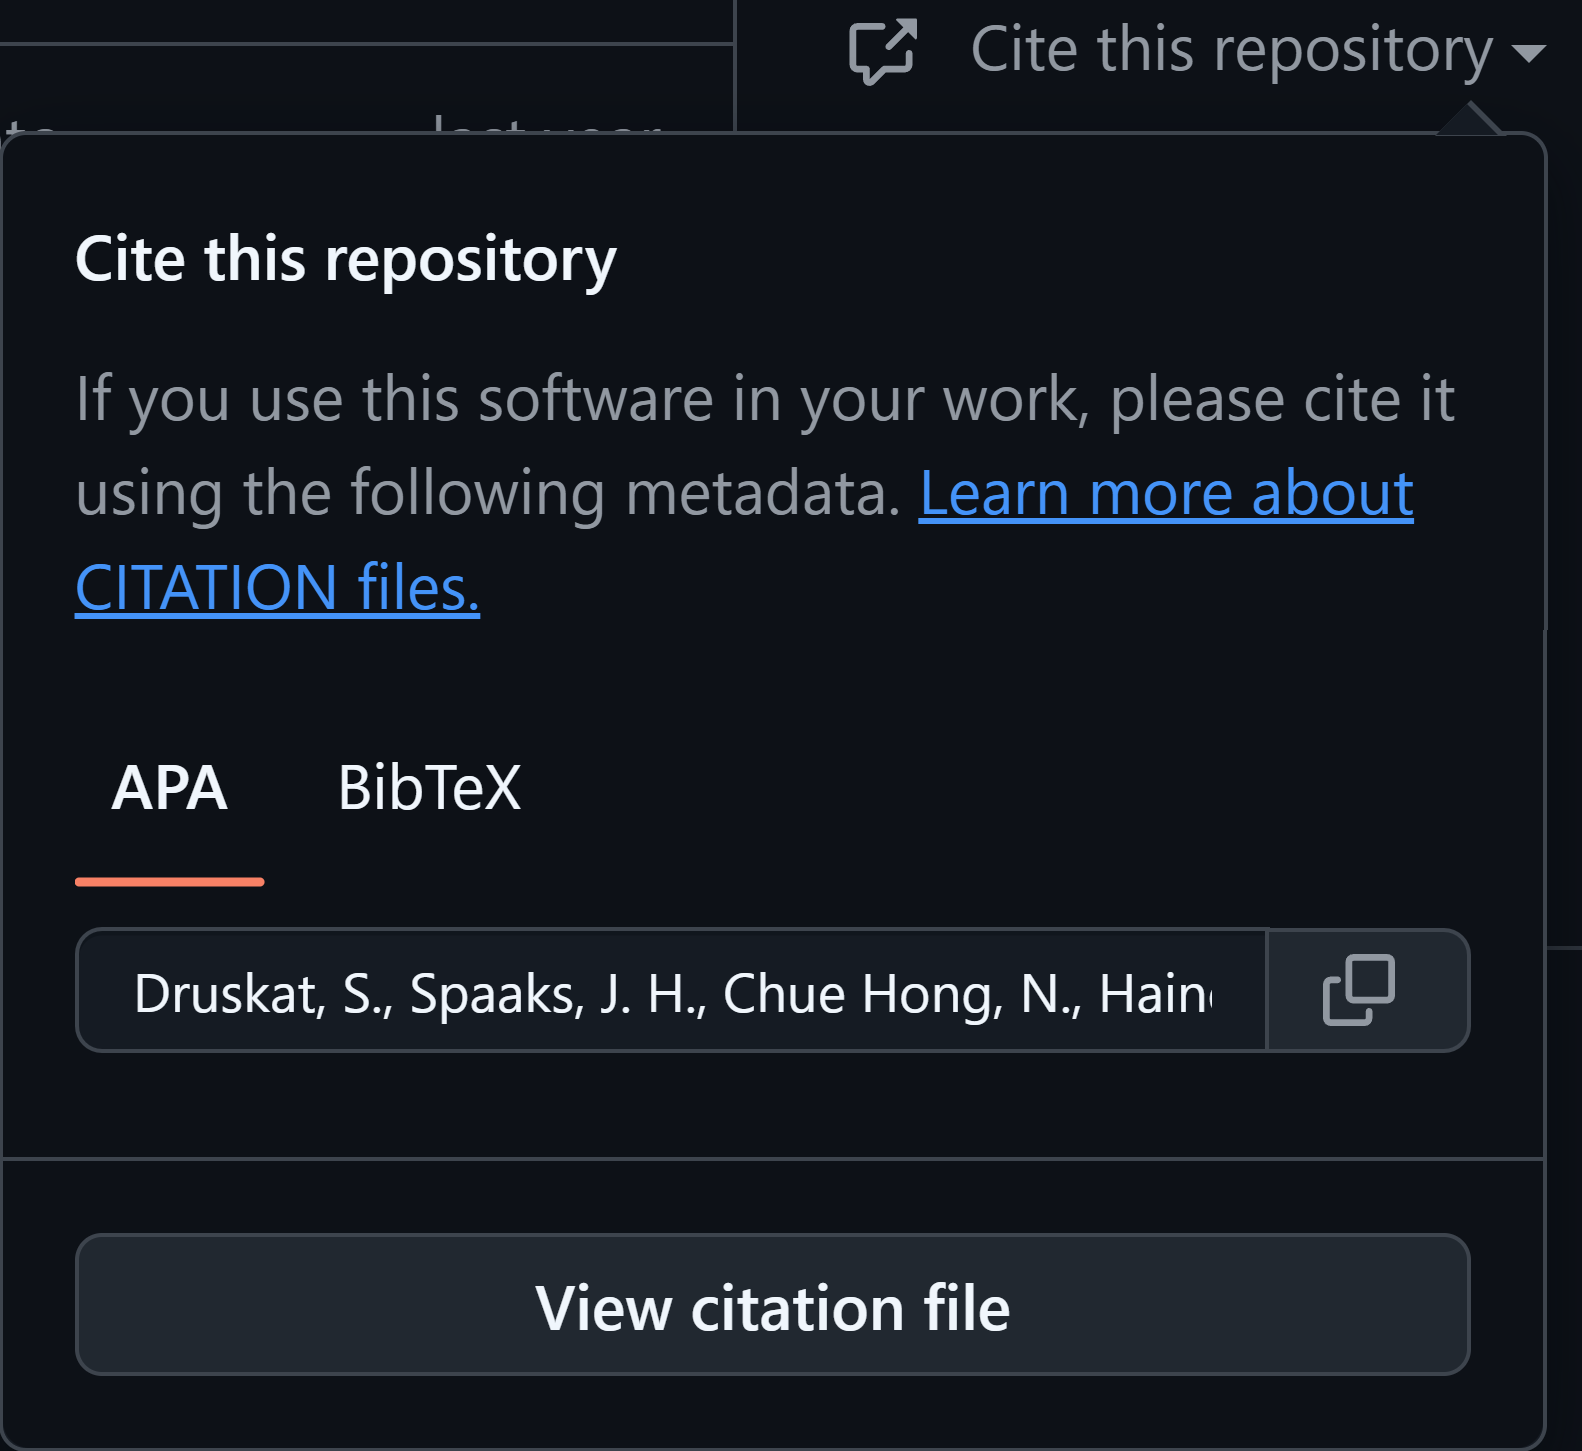
\includegraphics[width=0.5\textwidth]{bilder/GH_CFF_link.png}
    \end{center}
    \caption{GitHub-Repository mit \mintinline{text}{CITATION.cff}-Datei}
    \label{fig:gh_cff_link}
    \small
    Die Abbildung stellt den Link auf die \mintinline{text}{CITATION.cff}-Datei dar, wie ihn GitHub aktuell darstellt.
    Außerdem ist die Möglichkeit sichtbar, die Datei im \hologo{BibTeX}-Format und in der APA-Zitierweise zu kopieren \autocite{druskat_citation_2021-1}.
\end{figure}

In dem \gls{cff} existieren verschiedene Felder, welche für die Zitation von Software relevant sind.
Das wichtigste Feld ist das \emph{authors}-Feld, welches die Autoren der Software enthält und zwingend erforderlich ist.
In diesem Feld können die Autoren als Liste angegeben werden.
Ein Autor ist dabei entweder eine Person oder eine Entität.
Eine Entität kann beispielsweise eine Organisation sein.
Die Entität kann mit einem Namen mittels \emph{name} angegeben werden \autocite{druskat_citation_2021}.
Sie kann ebenfalls eine OORCID iD und eine E-Mail-Adresse enthalten.
Besonders wichtig für diese Arbeit ist die Referenz auf eine Person, da dies die einzige Information ist, welche aus Git extrahiert werden kann.
Eine Person enthält ebenfalls die genannten Werte einer Entität und wird jedoch über den Vor- und Nachname separiert mittels \emph{given-names} und \emph{family-names} angegeben.
Dadurch ist es möglich, die Personen von den Entitäten zu unterscheiden.

Ein weiteres Feld ist das \emph{preferred-citation}-Feld.
Mit diesem Feld ist es möglich, die Anerkennung für die Arbeit auf eine andere Arbeit zu übertragen \autocite{druskat_citation_2021}.
Ein Beispiel hierfür ist ein Paper über die Software, welches bevorzugt zitiert werden soll, anstelle der eigentlichen Software.
Hierbei können ebenfalls Personen und Entitäten angegeben werden.
Durch die Angabe einer \emph{preferred-citation} kann das Prinzip der Wichtigkeit vernachlässigt werden.
Auf dieses Verhalten wird in der Diskussion konkreter eingegangen.

Weitere in dieser Arbeit verwendete Felder sind \emph{type}, \emph{year}, \emph{month}, \emph{date-released}, \emph{date-published}, \emph{doi}, \emph{collection-doi} und \emph{identifiers}.
Das Feld \emph{type} ist zwingend erforderlich, hat jedoch als Standardwert \glqq software\grqq{}, sodass dies nicht angegeben werden muss.
Es gibt an, ob es sich um eine Software oder einen Datensatz handelt.
Dabei sind lediglich die Werte \glqq software\grqq{} oder \glqq dataset\grqq{} erlaubt.
Das Feld \emph{date-released} gibt an, wann die Software oder der Datensatz veröffentlicht wurde.
Das Feld \emph{doi} kann einen \glsdisp{doi}{Digitalen Objektbezeichner (DOI)} der Software oder des Datensatzes enthalten.
Mittels \emph{identifiers} können weitere Identifikatoren angeführt werden, wie z.~B. eine \gls{doi} oder eine URL, wobei die \emph{identifiers} mit einer Beschreibung erweitert werden können.
Die beschriebenen Felder können zusätzlich alle unter dem Feld \emph{preferred-citation} angegeben werden, um eine andere Arbeit zu referenzieren.

Die Felder \emph{year}, \emph{month} und \emph{date-published} können zusätzlich zu dem Feld \emph{date-released} unter dem Feld \emph{preferred-citation} angeführt werden, um das Jahr und das Datum der Veröffentlichung anzugeben.
Außerdem können weitere Typen mittels \emph{type} aufgeführt werden, wie beispielsweise \glqq thesis\grqq{} oder \glqq manual\grqq{}, sodass diese Arbeiten ebenfalls referenziert werden können.
Zusätzlich kann das Feld \emph{collection-doi} verwendet werden, um auf eine Sammlung von Arbeiten zu verweisen, die die Arbeit enthält.
Ein Beispiel einer \mintinline{text}{CITATION.cff}-Datei ist in \autoref{lst:cff_example} dargestellt.
Dabei wurde sich auf die beschriebenen und notwendigen Felder beschränkt.

\begin{listing}
    \inputminted{yaml}{../CITATION.cff}
    \caption{Beispiel einer \mintinline{text}{CITATION.cff}-Datei}
    \label{lst:cff_example}
    \small
    In dem Listing ist die \gls{cff}-Datei dieser Arbeit dargestellt. Dabei wurden primär Felder angegeben, welche in der Masterarbeit verwendet werden.
\end{listing}

\subsection{\hologo{BibTeX}}
\label{subsec:bibtex_format}
\hologo{BibTeX} ist eine Software, welche zur Erstellung von Literaturangaben und -verzeichnissen in \LaTeX{}-Dokumenten verwendet wird.
Außerdem existiert mit \hologo{BibTeX} ein gleichnamiges Format, welches in der \mintinline{text}{CITATION.bib}-Datei gespeichert wird und auf keinem anderen Format basiert.
\hologo{BibTeX} ist ein weit verbreiteter Standard und wird von vielen Autoren in der Wissenschaft verwendet.
Auf GitHub enthalten 2.144 Repositorys eine \mintinline{text}{CITATION.bib}-Datei (Stand 07.11.2024).
Das Format beschreibt die Zitation von Literatur und kann von Menschen und Maschinen gelesen werden.
Es beschränkt sich dabei nicht auf eine spezielle Art von Literatur, sondern kann für viele unterschiedliche Arten von Literatur verwendet werden.
Beispielsweise können Bücher und Masterarbeiten in \hologo{BibTeX} zitiert werden \autocite{patashnik_bibtexing_1988}.
Ein offizieller Literaturtyp für Software existiert nicht.
In der Datei können mehrere Einträge vorhanden sein, wobei jeder Eintrag eine Literaturangabe darstellt.

\hologo{BibTeX}-Dateien können von Menschen manuell erstellt und in das Repository eingebunden werden.
Außerdem existieren viele Literaturverwaltungsprogramme wie Zotero, welche \hologo{BibTeX}-Dateien erstellen und verarbeiten können \autocite{zotero_zotero_2024}.
Ebenfalls ist die Integration in andere Plattformen möglich, wie z.~B. in GitHub.
Hier wird die \mintinline{text}{CITATION.bib}-Datei auf der Repository-Startseite verlinkt, sie lässt sich jedoch im Gegensatz zu dem \gls{cff} nicht direkt kopieren oder in andere Formate umwandeln \autocite{github_about_2024-1}.

In dem \hologo{BibTeX}-Format existieren verschiedene Felder, welche für die Zitation von Literatur relevant sind.
Welche Felder zwingend erforderlich sind, hängt vom jeweiligen Literaturtyp ab.
Zudem sind die verfügbaren Felder ebenfalls vom Literaturtyp abhängig \autocite{patashnik_bibtexing_1988}.
In dieser Arbeit wird auf einige dieser Felder eingegangen, welche für die spätere Auswertung relevant sind.
Das wichtigste Feld ist das \emph{author}-Feld, welches die Autoren der Literatur enthält und zwingend erforderlich ist.
Die Vor- und Nachnamen der Autoren werden mit einem Komma separiert und mehrere Autoren werden über ein \glqq and\grqq{} getrennt.
Weitere Felder, welche für die Masterarbeit verwendet werden, sind \emph{year} und \emph{month}, welche das Jahr und den Monat der Veröffentlichung angeben.
Ein Beispiel einer \mintinline{text}{CITATION.bib}-Datei ist in \autoref{lst:bibtex_example} dargestellt.
Es ist zu erkennen, dass in dem \hologo{BibTeX}-Eintrag Informationen fehlen, welche in dem \gls{cff}-Eintrag vorhanden waren.
Dies liegt daran, dass in dem \hologo{BibTeX}-Eintrag nur eine Referenz auf die Masterarbeit möglich ist und nicht auf die entwickelte Software.

\begin{listing}
  \inputminted{text}{../CITATION.bib}
  \caption{Beispiel einer \mintinline{text}{CITATION.bib}-Datei}
  \label{lst:bibtex_example}
  \small
  In dem Listing ist die \hologo{BibTeX}-Datei dieser Arbeit dargestellt. Dabei wurden primär Felder angegeben, welche in der Masterarbeit verwendet werden.
\end{listing}

\section{Named Entity Recognition}
\label{sec:named-entity-recognition}

\section{Named Entity Disambiguation}
\label{sec:author-name-disambiguation}
% TODO ggf. noch weiter ausführen?
Die \gls{ned} ist ein automatischer Prozess, bei dem ein Name einer Entität einer gegebenen Datenmenge zugeordnet wird \autocites{cucerzan_large-scale_2007}{yamada_global_2022}.
Die Entitäten können beispielsweise durch die \gls{ner} extrahiert worden sein.
Dabei kann es dazu kommen, dass eine Entität mehrfach extrahiert wird und mehrfach in der Datenmenge vorhanden ist, jedoch mit anderen Bedeutungen.
In der natürlichen Sprachverarbeitung ist dies das Problem der Polysemie.
Es ist aber auch möglich, dass Personen mit dem gleichen Namen, sogenannte Namensvetter extrahiert werden, welche unterschieden werden müssen.
Dies beschreibt die Author name disambiguation, welche konkret individuelle Personen disambiguiert und ein Teil der \gls{ned} ist.
Diese Probleme kann die \gls{ned} mittels Modellen lösen, die die Entitäten anhand von Kontexten disambiguieren.
Beispiele für erkannte Entitäten sind \autocite{cucerzan_large-scale_2007}:

\begin{itemize}
  \item George W. Bush (George W. Bush)
  \item George Bush (George W. Bush)
  \item Bush (George W. Bush)
  \item Reggie Bush (Reggie Bush)
  \item Bush (Reggie Bush)
  \item Bush (Rock band)
\end{itemize}

In dem Beispiel ist die Entität dargestellt, gefolgt von der Entität in der Datenmenge, welche in Klammern steht.
Hierbei ist auffällig, dass Nennungen von \glqq Bush\grqq{} mehrfach vorkommen und durch den Kontext, in dem sie stehen, durch die \gls{ned} unterschieden werden müssen.

\gls{ned} wird in vielen Bereichen eingesetzt, wie z.~B. Textanalysen, semantische Suche und der Gruppierung von Software-Nennungen in wissenschaftlichen Arbeiten \autocites{cucerzan_large-scale_2007}{yamada_global_2022}{schindler_somesci-_2021}.
In dieser Masterarbeit kann die \gls{ned} verwendet werden, um Autoren aus verschiedenen Quellen miteinander abzugleichen.

Ähnlich zu der \gls{ner} gibt es für die \gls{ned} verschiedene Modelle.
Viele Modelle sind jedoch spezifisch auf einzelne Aufgabenbereiche trainiert.
Allgemeine Modelle sind primär für die Disambiguierung von Entitäten in Texten trainiert, welche in dieser Arbeit nicht immer vorhanden sind.
Ein Beispiel ist ein Modell von Yamade u.~a., welches Wörter, sowohl als auch Entitäten als Tokens erhält und diese mit Entitäten aus einem Text disambiguiert \autocite{yamada_global_2022}.

\section{Unscharfe Suche}
\label{sec:unscharfe-suche}
% TODO ggf. Levenshtein Distance und Damerau-Levenshtein-Distanz leicht erklären
% TODO ggf. noch weiter ausführen?
Die unscharfe Suche ist ein Verfahren, um ähnliche Zeichenfolgen zu finden, die sich in ihrer Schreibweise unterscheiden \autocite{hall_approximate_1980}.
Dieses Verfahren hat viele Anwendungsgebiete in der Informatik.
Ein Beispiel ist das Finden eines Personennamens in einem Index.
Falls der Name exakt in dem Index vorhanden ist, ist die Suche trivial.
Falls der Name unterschiedlich geschrieben ist, beispielsweise durch Abkürzungen oder Tippfehler, schlägt die triviale Suche fehl.
Die unscharfe Suche kann in diesem Fall helfen, den Namen dennoch zu finden.
Ein weiteres Anwendungsgebiet ist eine allgemeine Suche, beispielsweise von Produkten in einem Online-Shop.
Hierbei müssen auch Tippfehler berücksichtigt werden.

Die unscharfe Suche kann auf der Levenshtein-Distanz basieren \autocite{levenshtein_binary_1965}.
Als Ergebnis der unscharfen Suche wird in vielen Implementierungen die Distanz zwischen zwei Zeichenfolgen in Prozent angegeben.
Die Levenshtein-Distanz verwendet drei Arten von einzelzeichenbasierten Editieroperationen, um die Distanz zwischen zwei Zeichenfolgen zu berechnen.

\begin{enumerate}
    \item Einfügen eines Zeichens zur Zeichenfolge (Suhe \rightarrow{} Su\textbf{c}he)
    \item Löschen eines Zeichens aus der Zeichenfolge (Suche\textbf{e} \rightarrow{} Suche)
    \item Ersetzen eines Zeichens in der Zeichenfolge (S\textbf{i}che \rightarrow{} S\textbf{u}che)
\end{enumerate}

Zusätzlich zu der Levenshtein-Distanz existiert eine Erweiterung, die Damerau-Levenshtein-Distanz \autocite{damerau_technique_1964}.
Diese erweitert die Levenshtein-Distanz um eine vierte Editieroperation.
Mittels dieser vier Operationen werden ungefähr 80 \% der menschlichen Tippfehler abgedeckt \autocite{damerau_technique_1964}.

\begin{enumerate}
    \setcounter{enumi}{3}
    \item Vertauschen von zwei benachbarten Zeichen in der Zeichenfolge (Su\textbf{hc}e \rightarrow{} Su\textbf{ch}e)
\end{enumerate}

Eine Herausforderung bei der unscharfen Suche ist die Laufzeit.
Sie ist ungefähr proportional zum Produkt der beiden Zeichenfolgenlängen, wodurch eine unscharfe Suche nach langen Zeichenfolgen unpraktisch wird.
Eine weitere Herausforderung ist das Finden des richtigen Prozentsatzes, um die unscharfe Suche zu verwenden.
Ein zu hoher Prozentsatz führt dazu, dass die Suche zu viele Ergebnisse zurückgibt, während ein zu niedriger Prozentsatz dazu führt, dass die Suche zu wenige Ergebnisse zurückgibt.

Für die unscharfe Suche gibt es viele Implementierungen, die auf verschiedenen Algorithmen basieren.
Ein Programm, welches in Python implementiert ist, ist \emph{TheFuzz} \autocite{bachmann_thefuzz_2023}.
Das Programm basiert auf \emph{RapidFuzz}, welches die Levenshtein-Distanz in Python und C++ implementiert \autocites{bachmann_rapidfuzz_2023}.

